\section{Fully Supervised Approach}\label{fully_supervised_approach}
In this last section we follow the same steps of \Cref{hybrid_model_tuning,hybrid_pipeline_evaluation}, referring now
to the true labels from the dataset. Again, I relied on a 5-fold cross validation in order to tune different configurations for each model,
comparing the performance in terms of both balanced accuracy and computational cost. Since the hyperparamter grids were the same as the 
ones used in the previous section, I will report directly the best configurations:
\begin{itemize}
    \item \textbf{SVC}: gaussian kernel, with gamma=0.01 and C=10;
    \item \textbf{FCNN}: 512 hidden units, ReLU non linearity and dropout rate of 0.5, trained with 
    a learning rate of 0.01 and a batch size of 256;
    \item \textbf{CNN}:  ReLU non linearity, AvgPool2d pooling and batch normalization, trained with
    a learning rate of 0.01 and a batch size of 64.
\end{itemize}
Results from cross validation are summarized in \Cref{tab:model_comparison_FullySupervised}, 
while the performance on the test set is presented in \Cref{fig:confusion_matrices_FullySupervised,tab:ClassificationReport_FullySupervised}.

\begin{table}[h!]
    \centering
    \begin{adjustbox}{max width=0.85\textwidth}
    \begin{tabular}{|l|c|c|c|}
    \hline
    \textbf{Model} & \textbf{Balanced Accuracy} & \textbf{Training Time (s)} & \textbf{Inference Time (s)}  \\
    \hline
    SVC & 0.8656  $\pm$ 0.0070 & 1.5808 $\pm$ 0.0108 & 1.1168 $\pm$ 0.0046 \\
    FCNN & 0.8424 $\pm$ 0.0046 & 2.5826 $\pm$ 0.1118 & 0.0107 $\pm$ 0.0034 \\
    CNN & 0.8158  $\pm$ 0.0085 & 5.4935 $\pm$ 0.0034 & 0.0497 $\pm$ 0.0000 \\
    \hline
    \end{tabular}
    \end{adjustbox}
    \caption{\footnotesize Comparison of SVC, FCNN, and CNN in terms of balanced accuracy, training time, and inference time. 
    All the values are expressed as confidence intervals at 95\% level.}
    \label{tab:model_comparison_FullySupervised}
\end{table}

\begin{figure}[!htb]
    \begin{minipage}{0.33\textwidth}
      \centering
      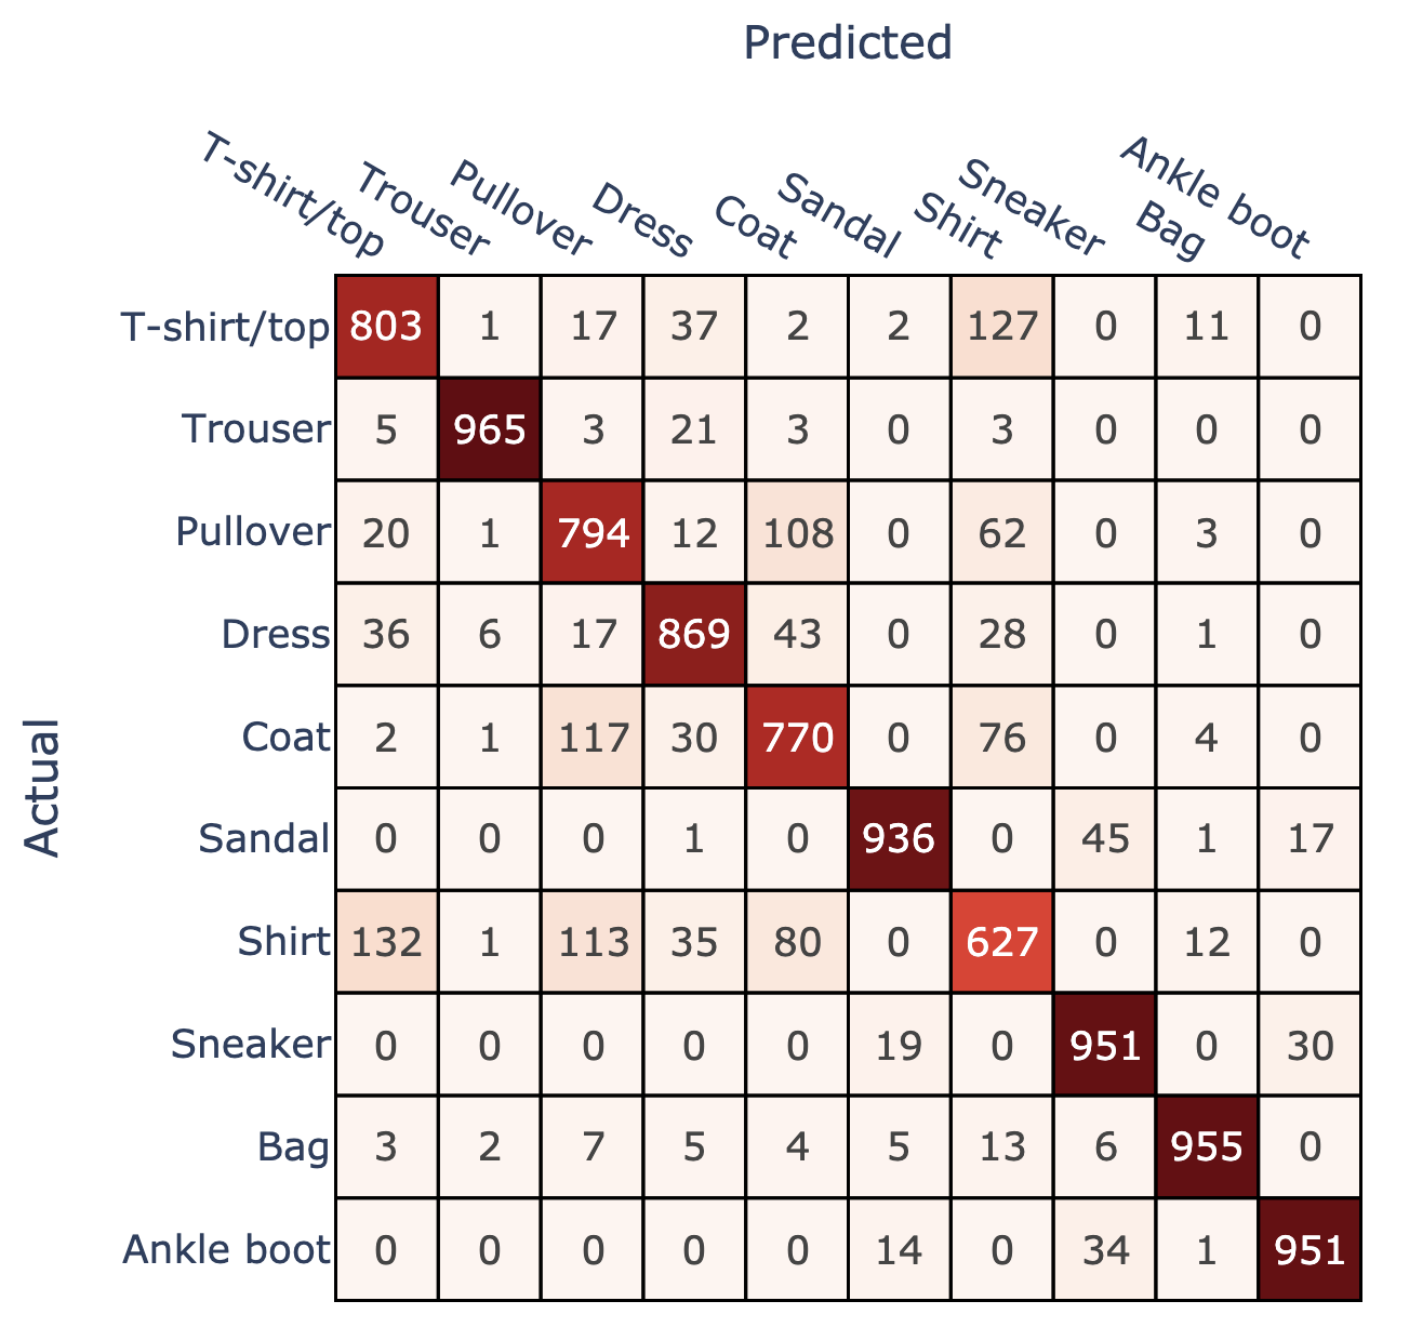
\includegraphics[width=1\linewidth]{images/CM_FullySupervised_SVC.png}
      \subcaption{\footnotesize SVC}
    \end{minipage}\hfill
    \begin{minipage}{0.33\textwidth}
      \centering
      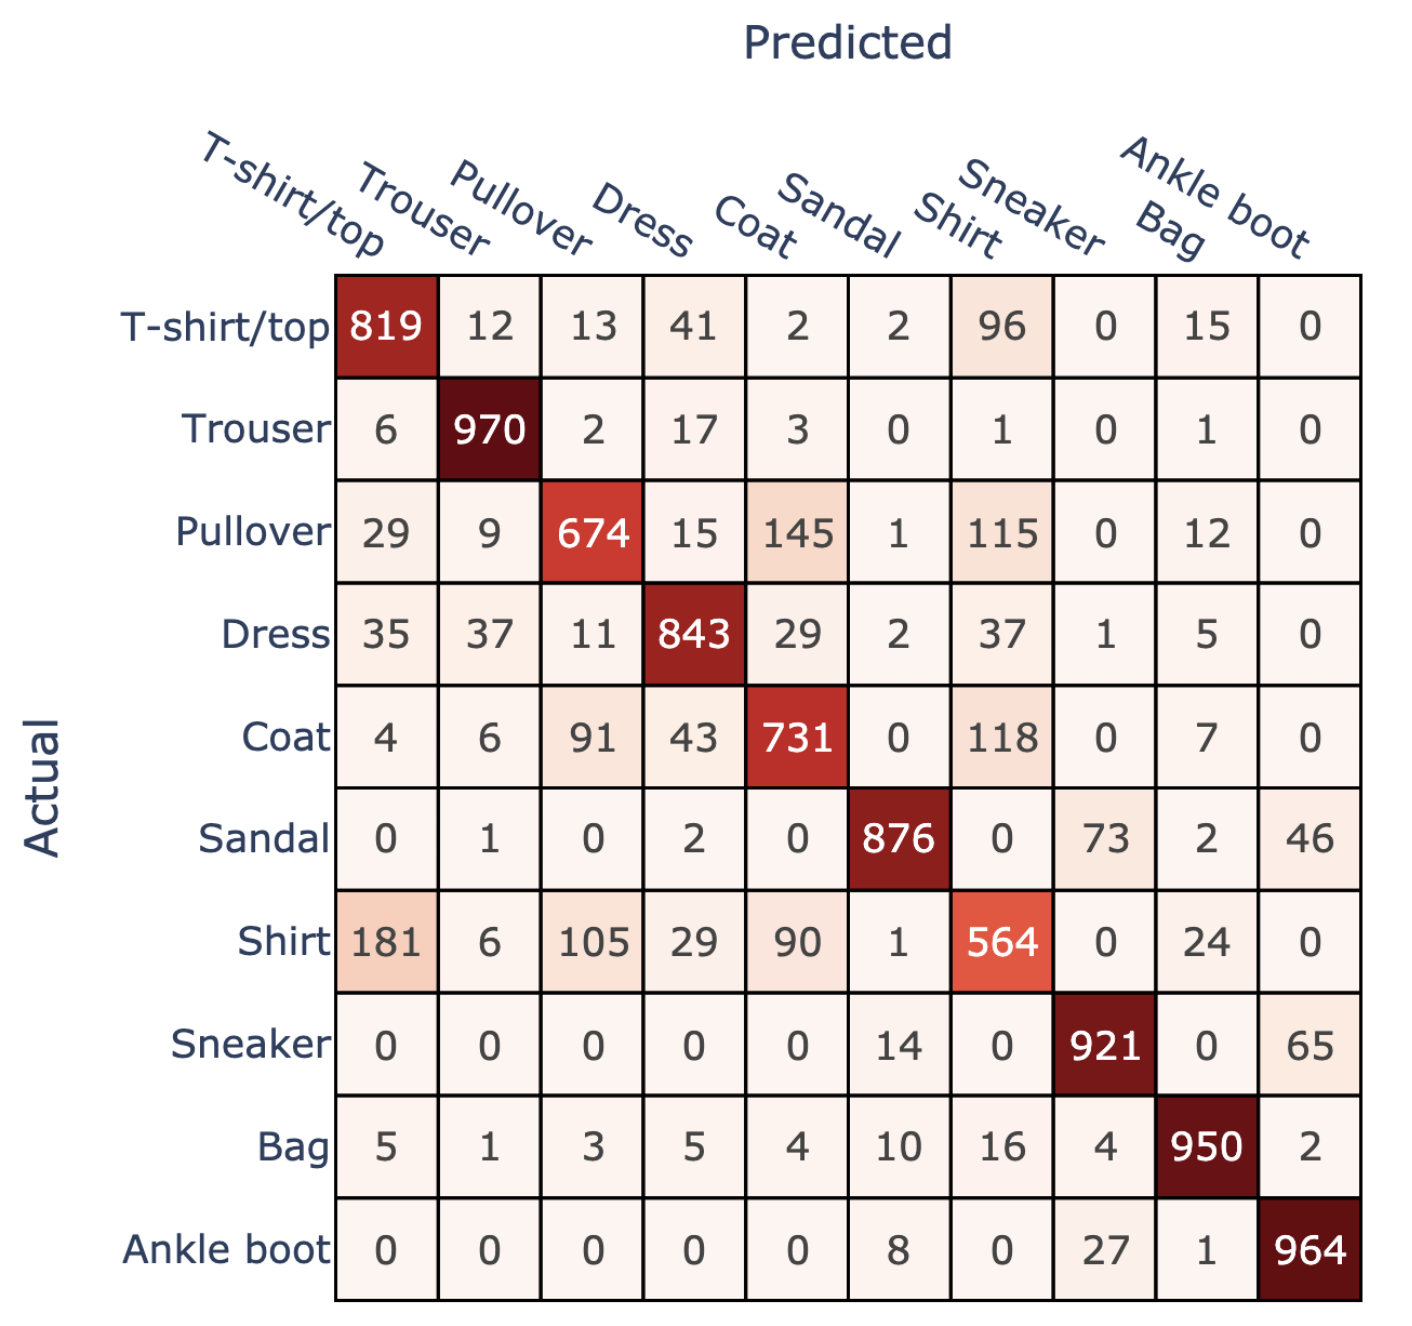
\includegraphics[width=1\linewidth]{images/CM_FullySupervised_FCNN.png}
      \subcaption{\footnotesize FCNN}
    \end{minipage}\hfill
    \begin{minipage}{0.33\textwidth}
        \centering
        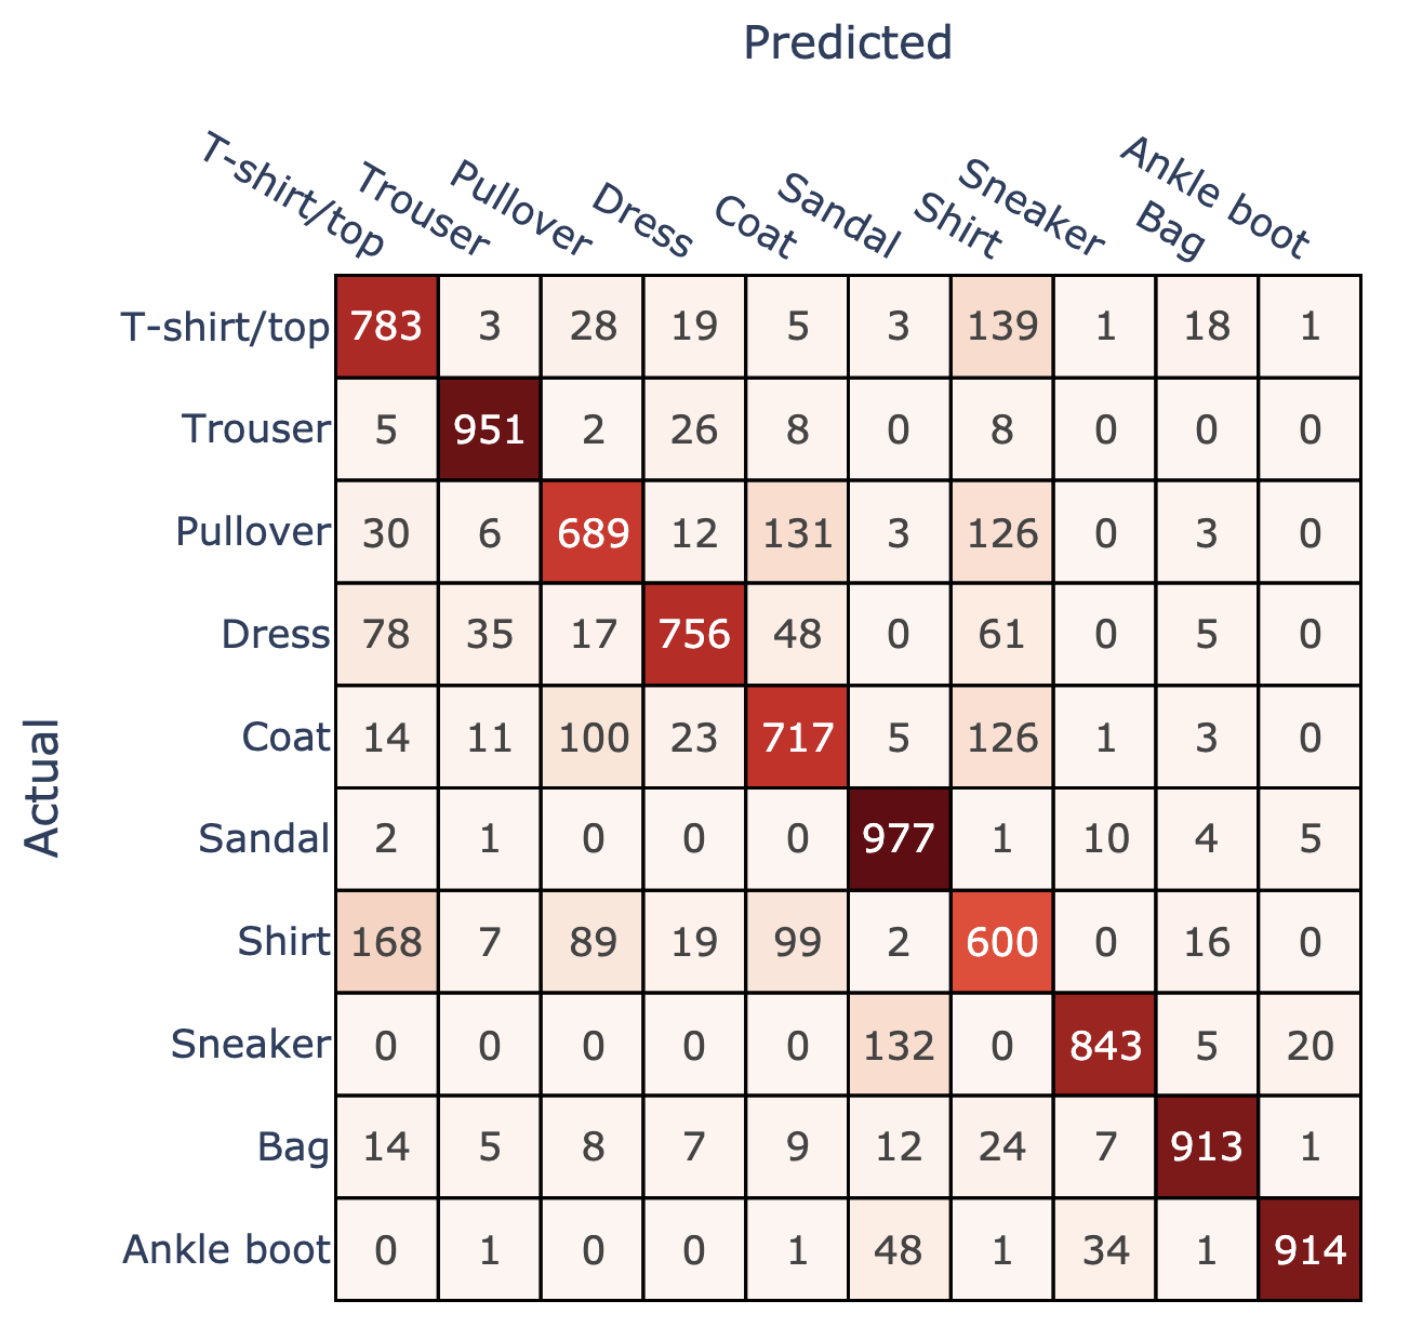
\includegraphics[width=1\linewidth]{images/CM_FullySupervised_CNN.png}
        \subcaption{\footnotesize CNN}
    \end{minipage}
    \caption{\footnotesize Confusion matrices for classification models [Fully Supervised Approach]}
    \label{fig:confusion_matrices_FullySupervised}
 \end{figure}


 \begin{table}[H]
    \centering
    \begin{minipage}{0.32\textwidth}
        \centering
        \begin{adjustbox}{max width=1\textwidth}
            \begin{tabular}{|c|c|c|c|}
                \hline
                \textbf{Class}     & \textbf{Precision} & \textbf{Recall} & \textbf{F1-Score} \\ \hline
                Ankle boot         & 0.95               & 0.95            & 0.95              \\
                Bag                & 0.97               & 0.95            & 0.96              \\
                Coat               & 0.76               & 0.77            & 0.77              \\
                Dress              & 0.86               & 0.87            & 0.86              \\
                Pullover           & 0.74               & 0.79            & 0.77              \\
                Sandal             & 0.96               & 0.94            & 0.95              \\
                Shirt              & 0.67               & 0.63            & 0.65              \\
                Sneaker            & 0.92               & 0.95            & 0.93              \\
                T-shirt/top        & 0.80               & 0.80            & 0.80              \\
                Trouser            & 0.99               & 0.96            & 0.98              \\ \hline
            \end{tabular}
        \end{adjustbox}
        \subcaption{\footnotesize SVC}
    \end{minipage}
    \hfill
    \begin{minipage}{0.32\textwidth}
        \centering
        \begin{adjustbox}{max width=1\textwidth}
            \begin{tabular}{|c|c|c|c|}
                \hline
                \textbf{Class}     & \textbf{Precision} & \textbf{Recall} & \textbf{F1-Score} \\ \hline
                Ankle boot         & 0.90               & 0.96            & 0.93              \\
                Bag                & 0.93               & 0.95            & 0.94              \\
                Coat               & 0.73               & 0.73            & 0.73              \\
                Dress              & 0.85               & 0.84            & 0.85              \\
                Pullover           & 0.75               & 0.67            & 0.71              \\
                Sandal             & 0.96               & 0.88            & 0.92              \\
                Shirt              & 0.60               & 0.56            & 0.58              \\
                Sneaker            & 0.90               & 0.92            & 0.91              \\
                T-shirt/top        & 0.76               & 0.82            & 0.79              \\
                Trouser            & 0.93               & 0.97            & 0.95              \\ \hline
            \end{tabular}
        \end{adjustbox}
        \subcaption{\footnotesize FCNN}
    \end{minipage}
    \hfill
    \begin{minipage}{0.32\textwidth}
        \centering
        \begin{adjustbox}{max width=1\textwidth}
            \begin{tabular}{|c|c|c|c|}
                \hline
                \textbf{Class}     & \textbf{Precision} & \textbf{Recall} & \textbf{F1-Score} \\ \hline
                Ankle boot         & 0.97               & 0.91            & 0.94              \\
                Bag                & 0.94               & 0.91            & 0.93              \\
                Coat               & 0.70               & 0.72            & 0.71              \\
                Dress              & 0.88               & 0.76            & 0.81              \\
                Pullover           & 0.74               & 0.69            & 0.71              \\
                Sandal             & 0.83               & 0.98            & 0.90              \\
                Shirt              & 0.55               & 0.60            & 0.58              \\
                Sneaker            & 0.94               & 0.84            & 0.89              \\
                T-shirt/top        & 0.72               & 0.78            & 0.75              \\
                Trouser            & 0.93               & 0.95            & 0.94              \\ \hline
            \end{tabular}
        \end{adjustbox}
        \subcaption{\footnotesize CNN}
    \end{minipage}
    \caption{\footnotesize Classification reports for models [Fully Supervised Approach]}
    \label{tab:ClassificationReport_FullySupervised}
\end{table}

The models trained with the fully supervised approach exhibit significantly higher performance across all metrics if compared 
to their counterparts with ID-mapped labels. From a global perspective, the overall balanced accuracy of \emph{SVC}, \emph{FCNN} and \emph{CNN} 
increased to 0.86, 0.83, and 0.82, respectively. A notable improvement is also observed at a class level, where the values 
of precision, recall, and F1-score are generally higher than those obtained with the hybrid pipeline. This result is not 
particularly surprising and, in my opinion, can be attributed to two main factors. First, in the fully supervised approach, 
we fed the model with 728-pixel images, which inherently carry far more information than the 10-dimensional vectors used at the very 
beginning of the hybrid pipeline. The higher dimensionality allows the models to capture richer and more detailed patterns, significantly 
contributing to their superior performance. Second, the fully supervised approach involves training the models directly 
on the data, whereas the hybrid pipeline involves multiple stages, each introducing potential sources of error. During the 
dimensionality reduction phase, significant information loss occurs, as highlighted by the spectrum in \Cref{fig:kpa_spectrum}
and by the estimation of the manifold's intrinsic dimensionality. 
In the clustering phase, errors may occur if the algorithm fails to accurately represent the underlying structure of the data.
Besides the proposed dimensionality reduction method, I experimented with more advanced techniques such as t-SNE and UMAP, but 
these did not yield any significant improvement. My last trial was an AutoEncoder architecture, in order to leverage the 
encoder component to reduce data dimensionality. Although this approach made the cluster separation more distinct, 
it did not enhance classification performance. Finally, the mapping stage adds another layer of complexity, where issues can emerge from 
both the majority and the probabilistic mapping. These accumulated imperfections likely explain the performance gap between the 
two methods.\\[0.2cm]
From a qualitative perspective, trousers, ankle boots, sneakers, sandals, and dresses are consistently the best-classified labels. 
While the performance for other labels has improved, the models still struggle to correctly classify items such as shirts, coats, 
and pullovers. This observation aligns with the ones drawn in previous sections, proving our
pipeline to be valuable at least in gaining preliminary insights into the data structure.\\[0.2cm]
Interestingly, as in the hybrid approach, the model with the best performance is \emph{SVC}. This outcome surprised me a lot, 
as in the fully supervised setting, the model learns directly from the original images rather than from projections 
obtained through kernel-based dimensionality reduction. This suggests that the kernel trick applied to \emph{Fashion-MNIST} dataset may 
be particularly effective in mapping data points into a favorable feature space. However, it is crucial to point out that our 
analysis relied on a reduced slice of the dataset. If we were to train on the entire dataset, neural networks would significantly 
outperform \emph{SVC}, due to their ability to handle large datasets efficiently and effectively.



